\usetikzlibrary{patterns}


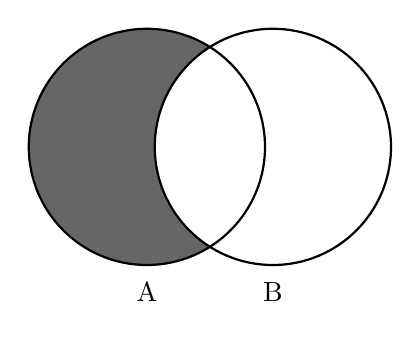
\begin{tikzpicture}[scale=1]

    % Define the radius for both circles
    \def\R{1.5}

    % Define the centers of circle A and circle B
    \coordinate (CenterA) at (0,0);
    \coordinate (CenterB) at (1.6,0);

    % Fill the area of A that does not intersect with B (A \setminus B)
    \begin{scope}
        % Restrict the drawing area to circle A
        \clip (CenterA) circle (\R);
        % Fill the entire circle A with a dark gray color to match the shaded region
        \fill[black!60] (CenterA) circle (\R);
        % Fill circle B with white to "erase" the overlapping area from the shading
        \fill[white] (CenterB) circle (\R);
    \end{scope}

    % Draw the outlines of circle A and circle B
    \draw[thick] (CenterA) circle (\R);
    \draw[thick] (CenterB) circle (\R);

    % Add the labels 'A' and 'B' below their respective circles
    \node[below] at (0,-1.6) {A};
    \node[below] at (1.6,-1.6) {B};

\end{tikzpicture}